
\usetikzlibrary{shapes,arrows}

% Definition of blocks:
\tikzset{%
  block/.style    = {draw, thick, rectangle, minimum height = 3em,
    minimum width = 3em},
  sum/.style      = {draw, circle, node distance = 2cm}, % Adder
  input/.style    = {coordinate}, % Input
  output/.style   = {coordinate} % Output
}
% Defining string as labels of certain blocks.
\newcommand{\suma}{\Large$+$}
\newcommand{\inte}{$\displaystyle \int$}
\newcommand{\derv}{\huge$\frac{d}{dt}$}

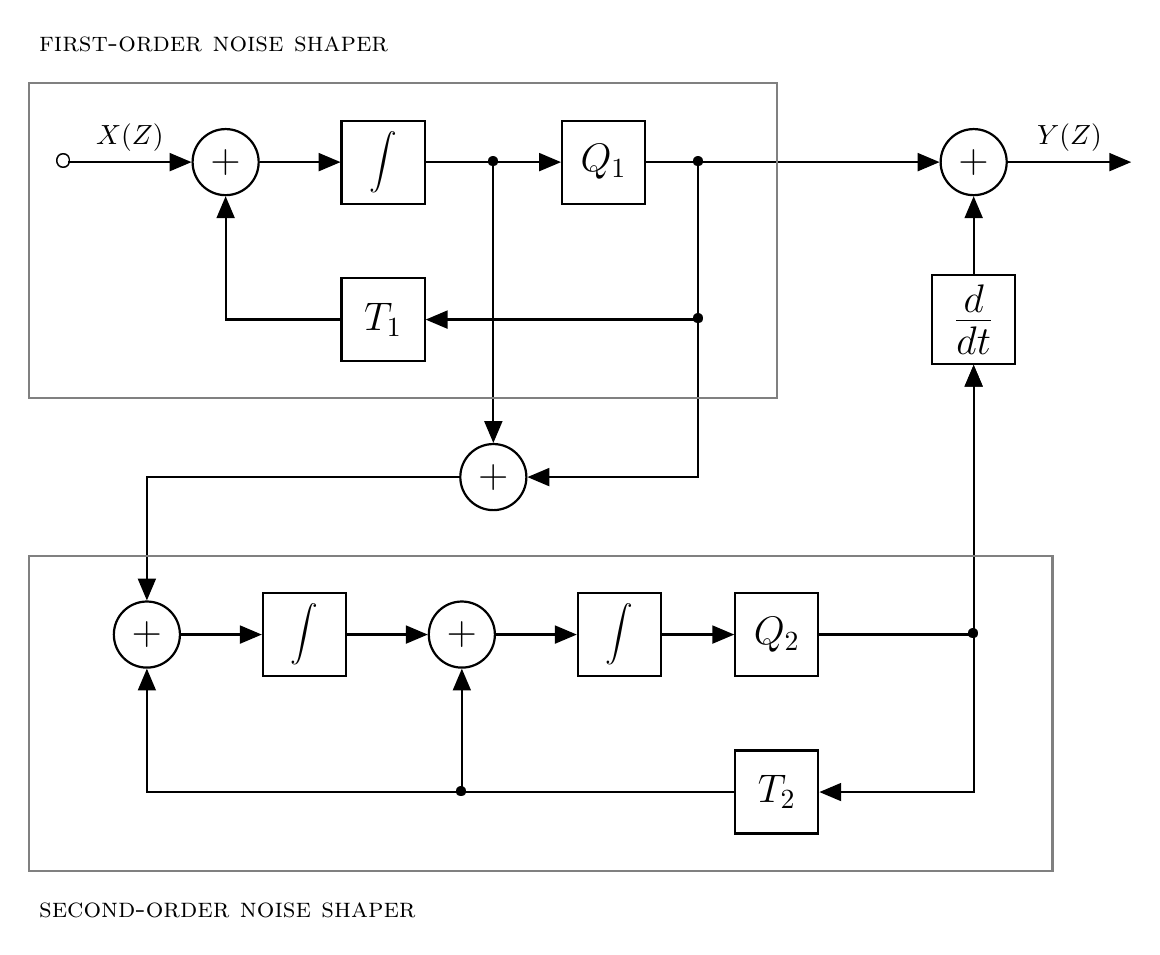
\begin{tikzpicture}[auto, thick, node distance=2cm, >=triangle 45]
\draw
	% Drawing the blocks of first filter :
	node at (0,0)[right=-3mm]{\Large \textopenbullet}
	node [input, name=input1] {} 
	node [sum, right of=input1] (suma1) {\suma}
	node [block, right of=suma1] (inte1) {\inte}
         node at (6.8,0)[block] (Q1) {\Large $Q_1$}
         node [block, below of=inte1] (ret1) {\Large$T_1$};
    % Joining blocks. 
    % Commands \draw with options like [->] must be written individually
	\draw[->](input1) -- node {$X(Z)$}(suma1);
 	\draw[->](suma1) -- node {} (inte1);
	\draw[->](inte1) -- node {} (Q1);
	\draw[->](ret1) -| node[near end]{} (suma1);
	% Adder
\draw
	node at (5.4,-4) [sum, name=suma2] {\suma}
    	% Second stage of filter 
	node at  (1,-6) [sum, name=suma3] {\suma}
	node [block, right of=suma3] (inte2) {\inte}
	node [sum, right of=inte2] (suma4) {\suma}
	node [block, right of=suma4] (inte3) {\inte}
	node [block, right of=inte3] (Q2) {\Large$Q_2$}
	node at (9,-8) [block, name=ret2] {\Large$T_2$}
;
	% Joining the blocks of second filter
	\draw[->] (suma3) -- node {} (inte2);
	\draw[->] (inte2) -- node {} (suma4);
	\draw[->] (suma4) -- node {} (inte3);
	\draw[->] (inte3) -- node {} (Q2);
	\draw[->] (ret2) -| (suma3);
	\draw[->] (ret2) -| (suma4);
         % Third stage of filter:
	% Defining nodes:
\draw
	node at (11.5, 0) [sum, name=suma5]{\suma}
	node [output, right of=suma5]{}
	node [block, below of=suma5] (deriv1){\derv}
	node [output, right of=suma5] (sal2){}
;
	% Joining the blocks:
	\draw[->] (suma2) -| node {}(suma3);
	\draw[->] (Q1) -- (8,0) |- node {}(ret1);
	\draw[->] (8,0) |- (suma2);
	\draw[->] (5.4,0) -- (suma2);
	\draw[->] (Q1) -- node {}(suma5);
	\draw[->] (deriv1) -- node {}(suma5);
	\draw[->] (Q2) -| node {}(deriv1);
    	\draw[<->] (ret2) -| node {}(deriv1);
    	\draw[->] (suma5) -- node {$Y(Z)$}(sal2);
    	% Drawing nodes with \textbullet
\draw
	node at (8,0) {\textbullet} 
	node at (8,-2){\textbullet}
	node at (5.4,0){\textbullet}
    	node at (5,-8){\textbullet}
    	node at (11.5,-6){\textbullet}
    	;
	% Boxing and labelling noise shapers
	\draw [color=gray,thick](-0.5,-3) rectangle (9,1);
	\node at (-0.5,1) [above=5mm, right=0mm] {\textsc{first-order noise shaper}};
	\draw [color=gray,thick](-0.5,-9) rectangle (12.5,-5);
	\node at (-0.5,-9) [below=5mm, right=0mm] {\textsc{second-order noise shaper}};
\end{tikzpicture}